\documentclass[11pt,a4paper]{report}
\usepackage[textwidth=37em,vmargin=30mm]{geometry}
\usepackage{calc,xunicode,amsmath,amssymb,paralist,enumitem,tabu,booktabs,datetime2,xeCJK,xeCJKfntef,listings}
\usepackage{tocloft,fancyhdr,tcolorbox,xcolor,graphicx,eso-pic,xltxtra,xelatexemoji}

\newcommand{\envyear}[0]{2025}
\newcommand{\envdatestr}[0]{2025-11-01}
\newcommand{\envfinaldir}[0]{webdb/2025/20251101/final}

\usepackage[hidelinks]{hyperref}
\hypersetup{
    colorlinks=false,
    pdfpagemode=FullScreen,
    pdftitle={Web Digest - \envdatestr}
}

\setlength{\cftbeforechapskip}{10pt}
\renewcommand{\cftchapfont}{\rmfamily\bfseries\large\raggedright}
\setlength{\cftbeforesecskip}{2pt}
\renewcommand{\cftsecfont}{\sffamily\small\raggedright}

\setdefaultleftmargin{2em}{2em}{1em}{1em}{1em}{1em}

\usepackage{xeCJK,xeCJKfntef}
\xeCJKsetup{PunctStyle=plain,RubberPunctSkip=false,CJKglue=\strut\hskip 0pt plus 0.1em minus 0.05em,CJKecglue=\strut\hskip 0.22em plus 0.2em}
\XeTeXlinebreaklocale "zh"
\XeTeXlinebreakskip = 0pt


\setmainfont{Brygada 1918}
\setromanfont{Brygada 1918}
\setsansfont{IBM Plex Sans}
\setmonofont{JetBrains Mono NL}
\setCJKmainfont{Noto Serif CJK SC}
\setCJKromanfont{Noto Serif CJK SC}
\setCJKsansfont{Noto Sans CJK SC}
\setCJKmonofont{Noto Sans CJK SC}

\setlength{\parindent}{0pt}
\setlength{\parskip}{8pt}
\linespread{1.15}

\lstset{
	basicstyle=\ttfamily\footnotesize,
	numbersep=5pt,
	backgroundcolor=\color{black!5},
	showspaces=false,
	showstringspaces=false,
	showtabs=false,
	tabsize=2,
	captionpos=b,
	breaklines=true,
	breakatwhitespace=true,
	breakautoindent=true,
	linewidth=\textwidth
}






\newcommand{\coverpic}[2]{
    % argv: itemurl, authorname
    Cover photo by #2~~(\href{#1}{#1})
}
\newcommand{\makeheader}[0]{
    \begin{titlepage}
        % \newgeometry{hmargin=15mm,tmargin=21mm,bmargin=12mm}
        \begin{center}
            
            \rmfamily\scshape
            \fontspec{BaskervilleF}
            \fontspec{Old Standard}
            \fontsize{59pt}{70pt}\selectfont
            WEB\hfill DIGEST
            
            \vfill
            % \vskip 30pt
            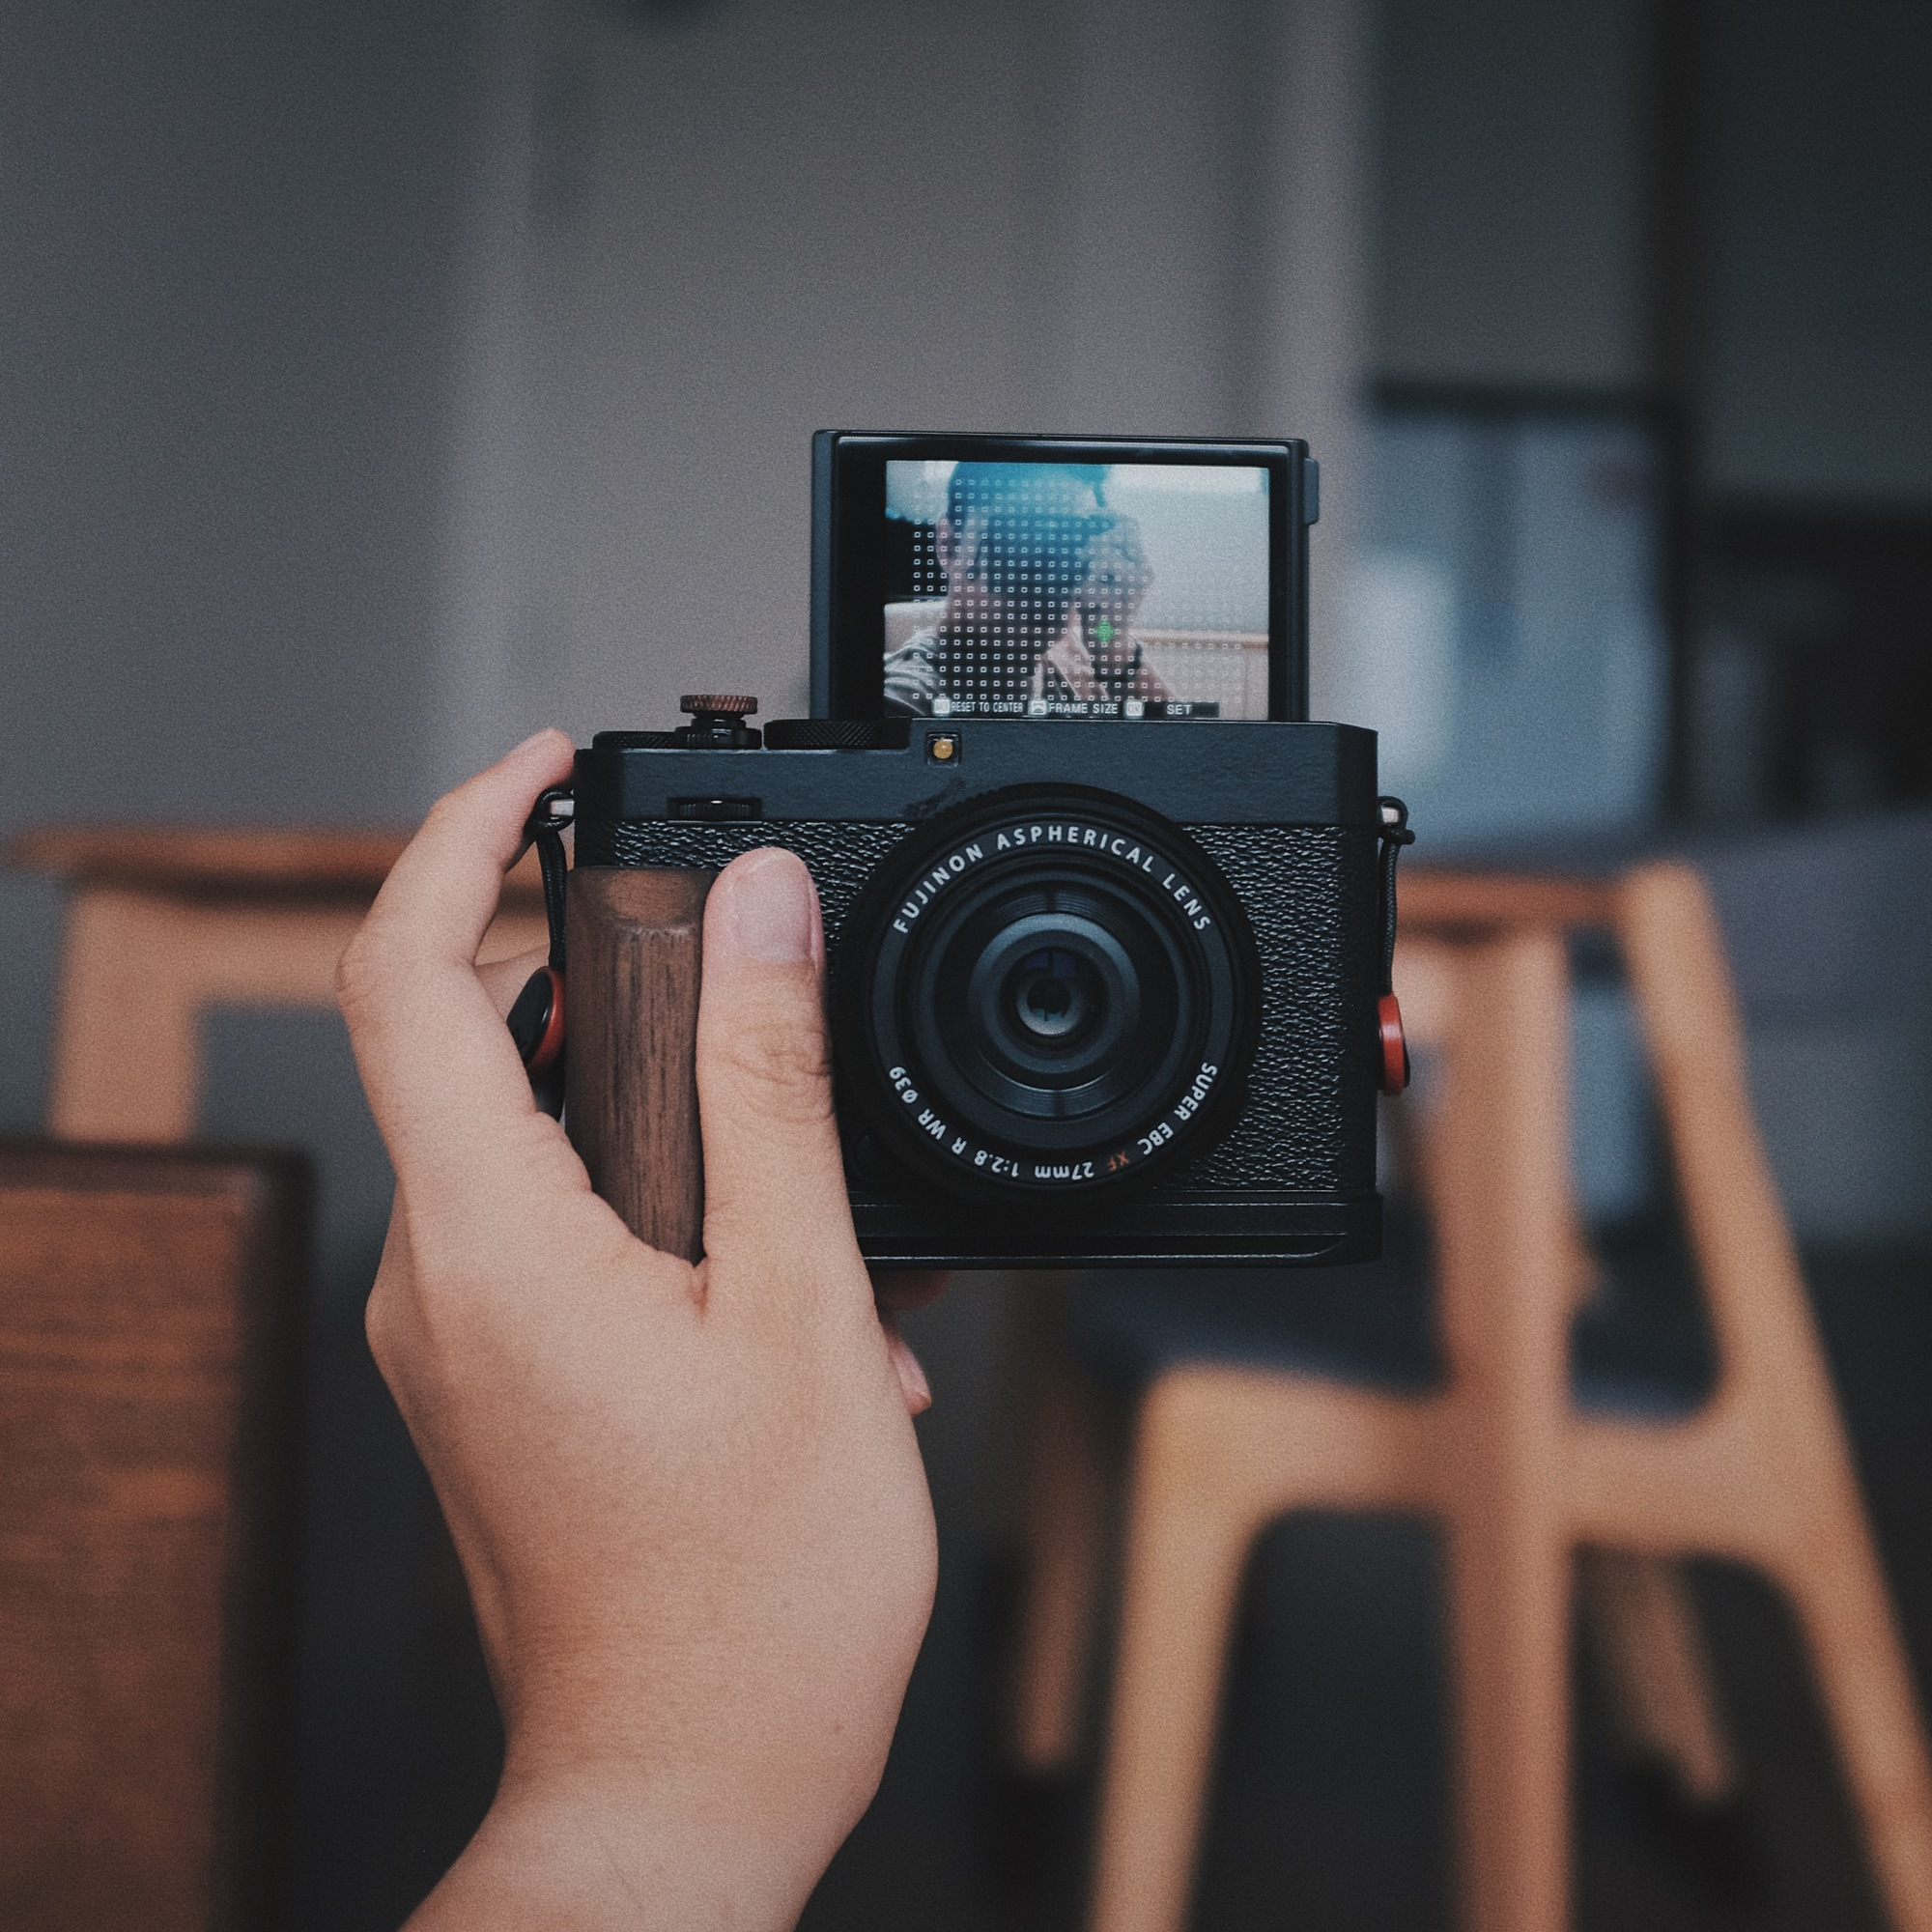
\includegraphics[width=\linewidth]{\envfinaldir/coverpic-prod.jpg}\par
            % \vskip 30pt
            \vfill

            \normalsize\rmfamily\scshape
            \copyright{} The Web Digest Project \hfill\large \envdatestr
        \end{center}
    \end{titlepage}
    % \restoregeometry
}
\newcommand{\simplehref}[1]{%
    \textcolor{blue!80!green}{\href{#1}{#1}}%
}
\renewcommand{\contentsname}{\center\Huge\sffamily\bfseries Contents\par\vskip 20pt}
\newcounter{ipartcounter}
\setcounter{ipartcounter}{0}
\newcommand{\ipart}[1]{
    % \vskip 20pt
    \clearpage
    \stepcounter{ipartcounter}
    \phantomsection
    \addcontentsline{toc}{chapter}{#1}
    % \begin{center}
    %     \Huge
    %     \sffamily\bfseries
    %     #1
    % \end{center}
    % \vskip 20pt plus 7pt
}
\newcounter{ichaptercounter}
\setcounter{ichaptercounter}{0}
\newcommand{\ichapter}[1]{
    % \vskip 20pt
    \clearpage
    \stepcounter{ichaptercounter}
    \phantomsection
    \addcontentsline{toc}{section}{\numberline{\arabic{ichaptercounter}}#1}
    \begin{center}
        \Huge
        \sffamily\bfseries
        #1
    \end{center}
    \vskip 20pt plus 7pt
}
\newcommand{\entrytitlefont}[1]{\subsection*{\raggedright\Large\sffamily\bfseries#1}}
\newcommand{\entryitemGeneric}[2]{
    % argv: title, url
    \parbox{\linewidth}{
        \entrytitlefont{#1}\par\vskip 5pt
        \footnotesize\ttfamily\mdseries
        \simplehref{#2}
    }\vskip 11pt plus 11pt minus 1pt
}
\newcommand{\entryitemGithub}[3]{
    % argv: title, url, desc
    \parbox{\linewidth}{
        \entrytitlefont{#1}\par\vskip 5pt
        \footnotesize\ttfamily\mdseries
        \simplehref{#2}\par\vskip 5pt
        \small\rmfamily\mdseries#3
    }\vskip 11pt plus 11pt minus 1pt
}
\newcommand{\entryitemAp}[3]{
    % argv: title, url, desc
    \parbox{\linewidth}{
        \entrytitlefont{#1}\par\vskip 5pt
        \footnotesize\ttfamily\mdseries
        \simplehref{#2}\par\vskip 5pt
        \small\rmfamily\mdseries#3
    }\vskip 11pt plus 11pt minus 1pt
}
\newcommand{\entryitemHackernews}[3]{
    % argv: title, hnurl, rawurl
    % \parbox{\linewidth}{
    %     \entrytitlefont{#1}\par\vskip 5pt
    %     \footnotesize\ttfamily\mdseries
    %     \simplehref{#3}\par
    %     \textcolor{black!50}{\href{#2}{#2}}
    % }\vskip 11pt plus 11pt minus 1pt
    \begin{minipage}{\linewidth}
            \entrytitlefont{#1}\par\vskip 5pt
            \footnotesize\ttfamily\mdseries
            \simplehref{#3}\par
            \textcolor{black!50}{\href{#2}{#2}}
    \end{minipage}\par\vskip 11pt plus 11pt minus 1pt
}







\begin{document}

\makeheader

\tableofcontents\clearpage




\ipart{Developers}
\ichapter{Hacker News}
\entryitemTwoLinks{Tim Bray on Grokipedia}{https://news.ycombinator.com/item?id=45777015}{https://www.tbray.org/ongoing/When/202x/2025/10/28/Grokipedia}

\entryitemTwoLinks{How to build silos and decrease collaboration on purpose}{https://news.ycombinator.com/item?id=45775642}{https://www.rubick.com/how-to-build-silos-and-decrease-collaboration/}

\entryitemTwoLinks{Addiction Markets}{https://news.ycombinator.com/item?id=45774640}{https://www.thebignewsletter.com/p/addiction-markets-abolish-corporate}

\entryitemTwoLinks{Use DuckDB-WASM to query TB of data in browser}{https://news.ycombinator.com/item?id=45774571}{https://lil.law.harvard.edu/blog/2025/10/24/rethinking-data-discovery-for-libraries-and-digital-humanities/}

\entryitemTwoLinks{Just use a button}{https://news.ycombinator.com/item?id=45774182}{https://gomakethings.com/just-use-a-button/}

\entryitemTwoLinks{Futurelock: A subtle risk in async Rust}{https://news.ycombinator.com/item?id=45774086}{https://rfd.shared.oxide.computer/rfd/0609}

\entryitemTwoLinks{Another European agency shifts off US Tech as digital sovereignty gains steam}{https://news.ycombinator.com/item?id=45773974}{https://www.zdnet.com/article/another-european-agency-ditches-big-tech-as-digital-sovereignty-movement-gains-steam/}

\entryitemTwoLinks{AI scrapers request commented scripts}{https://news.ycombinator.com/item?id=45773347}{https://cryptography.dog/blog/AI-scrapers-request-commented-scripts/}

\entryitemTwoLinks{Ubuntu Introduces Architecture Variants}{https://news.ycombinator.com/item?id=45772579}{https://lwn.net/Articles/1044383/}

\entryitemTwoLinks{Nix Derivation Madness}{https://news.ycombinator.com/item?id=45772347}{https://fzakaria.com/2025/10/29/nix-derivation-madness}

\entryitemTwoLinks{Nim 2.2.6}{https://news.ycombinator.com/item?id=45772224}{https://nim-lang.org//blog/2025/10/31/nim-226.html}

\entryitemTwoLinks{Immutable releases are now generally available on GitHub}{https://news.ycombinator.com/item?id=45772064}{https://github.blog/changelog/2025-10-28-immutable-releases-are-now-generally-available/}

\entryitemTwoLinks{Ask HN: Who uses open LLMs and coding assistants locally? Share setup and laptop}{https://news.ycombinator.com/item?id=45771870}{https://news.ycombinator.com/item?id=45771870}

\entryitemTwoLinks{Sustainable memristors from shiitake mycelium for high-frequency bioelectronics}{https://news.ycombinator.com/item?id=45771796}{https://journals.plos.org/plosone/article?id=10.1371/journal.pone.0328965}

\entryitemTwoLinks{Attention lapses due to sleep deprivation due to flushing fluid from brain}{https://news.ycombinator.com/item?id=45771636}{https://news.mit.edu/2025/your-brain-without-sleep-1029}

\entryitemTwoLinks{How OpenAI uses complex and circular deals to fuel its multibillion-dollar rise}{https://news.ycombinator.com/item?id=45771538}{https://www.nytimes.com/interactive/2025/10/31/technology/openai-fundraising-deals.html}

\entryitemTwoLinks{The cryptography behind electronic passports}{https://news.ycombinator.com/item?id=45770875}{https://blog.trailofbits.com/2025/10/31/the-cryptography-behind-electronic-passports/}

\entryitemTwoLinks{Claude outage}{https://news.ycombinator.com/item?id=45770317}{https://status.claude.com/incidents/s5f75jhwjs6g}

\entryitemTwoLinks{Reasoning models reason well, until they don't}{https://news.ycombinator.com/item?id=45769971}{https://arxiv.org/abs/2510.22371}

\entryitemTwoLinks{AMD could enter ARM market with Sound Wave APU built on TSMC 3nm process}{https://news.ycombinator.com/item?id=45767916}{https://www.guru3d.com/story/amd-enters-arm-market-with-sound-wave-apu-built-on-tsmc-3nm-process/}\ichapter{Phoronix}
\entryitemGeneric{\hskip 0pt{}GNOME Gains A New macOS-Inspired Quick Menu Option}{https://www.phoronix.com/news/GNOME-Kiwi-macOS-Quick-Menu}

\entryitemGeneric{\hskip 0pt{}KosmicKrisp Now Vulkan 1.3 Compliant For Apple Devices}{https://www.phoronix.com/news/KosmicKrisp-Vulkan-1.3}

\entryitemGeneric{\hskip 0pt{}Ubuntu 25.10 amd64v3 Benchmarks: Some Minor \& Rare Performance Advantages For Desktop Workloads}{https://www.phoronix.com/review/ubuntu-2510-amd64v3}

\entryitemGeneric{\hskip 0pt{}AMD Windows Driver Changes For RX 5000/6000 Series Won't Impact Linux Users}{https://www.phoronix.com/news/AMD-Windows-RX-5000-6000-Game}

\entryitemGeneric{\hskip 0pt{}Linux 6.18-rc4 Fixes Another Performance Regression In The Power Management Code}{https://www.phoronix.com/news/Linux-6.18-rc4-PM-Perf-Fix}

\entryitemGeneric{\hskip 0pt{}AerynOS 2025.10 ISOs Released - GNOME 49, Switches Back To GNU libstdc++}{https://www.phoronix.com/news/AerynOS-2025.10-ISOs}

\entryitemGeneric{\hskip 0pt{}Krita Lands Basic HDR Support On Wayland}{https://www.phoronix.com/news/Krita-HDR-Wayland-Support}

\entryitemGeneric{\hskip 0pt{}Vulkan 1.4.331 Brings Two New Extensions}{https://www.phoronix.com/news/Vulkan-1.4.331-Released}

\entryitemGeneric{\hskip 0pt{}Genode-Powered Sculpt OS 25.10 Brings Performance Improvements \& Better Drivers}{https://www.phoronix.com/news/Sculpt-OS-25.10-Released}


\ipart{Developers~~~~(zh-Hans)}
\ichapter{Solidot}
\entryitemGeneric{\hskip 0pt{}特朗普命令美国重启核武器试验}{https://www.solidot.org/story?sid=82688}

\entryitemGeneric{\hskip 0pt{}Bazzite 秋季更新释出}{https://www.solidot.org/story?sid=82687}

\entryitemGeneric{\hskip 0pt{}以色列要求 Google 和亚马逊使用秘密的眨眼信号警告外国政府的数据披露要求}{https://www.solidot.org/story?sid=82686}

\entryitemGeneric{\hskip 0pt{}英国面临禁止汞合金填充物的压力}{https://www.solidot.org/story?sid=82685}

\entryitemGeneric{\hskip 0pt{}Affinity Studio 成为免费软件 }{https://www.solidot.org/story?sid=82684}

\entryitemGeneric{\hskip 0pt{}数学证明否定宇宙是模拟的}{https://www.solidot.org/story?sid=82683}

\entryitemGeneric{\hskip 0pt{}DNS 运行在 FOSS 之上}{https://www.solidot.org/story?sid=82682}

\entryitemGeneric{\hskip 0pt{}社会最终会接受自动驾驶出租车导致的致命车祸}{https://www.solidot.org/story?sid=82681}

\entryitemGeneric{\hskip 0pt{}Meta 否认下载成人视频用于训练 AI,称只是``个人使用''}{https://www.solidot.org/story?sid=82680}

\entryitemGeneric{\hskip 0pt{}国际刑事法院抛弃微软软件}{https://www.solidot.org/story?sid=82679}

\entryitemGeneric{\hskip 0pt{}AOL 以 15 亿美元出售给 Bending Spoons}{https://www.solidot.org/story?sid=82678}

\entryitemGeneric{\hskip 0pt{}SUSE 成为第一个集成智能体的 Linux 企业发行版}{https://www.solidot.org/story?sid=82677}

\entryitemGeneric{\hskip 0pt{}微软 XBox 掌机存在大量 Windows 系统问题}{https://www.solidot.org/story?sid=82676}

\entryitemGeneric{\hskip 0pt{}Pop!\_OS 24.04 LTS 将于 12 月推出}{https://www.solidot.org/story?sid=82675}

\entryitemGeneric{\hskip 0pt{}Grammarly 改名为 Superhuman}{https://www.solidot.org/story?sid=82674}

\entryitemGeneric{\hskip 0pt{}Tor Browser 15.0 释出}{https://www.solidot.org/story?sid=82673}

\entryitemGeneric{\hskip 0pt{}Fedora Linux 43 释出}{https://www.solidot.org/story?sid=82672}

\entryitemGeneric{\hskip 0pt{}英伟达成为第一家市值突破 5 万亿美元的公司}{https://www.solidot.org/story?sid=82671}

\entryitemGeneric{\hskip 0pt{}小鼠研究显示头发在 20 天内完全再生}{https://www.solidot.org/story?sid=82670}

\entryitemGeneric{\hskip 0pt{}矮星系发现巨大黑洞}{https://www.solidot.org/story?sid=82669}\ichapter{V2EX}
\entryitemGeneric{\hskip 0pt{}[生活] 为女生发声\_驳斥「现在的女生月光、不存钱普遍吗?」}{https://www.v2ex.com/t/1169829}

\entryitemGeneric{\hskip 0pt{}[分享发现] 国内所有的视频网站,哪怕你开了 SSSSSVIP,也没有 5.1 或者 7.1 声道,更别提杜比和 DTS 了}{https://www.v2ex.com/t/1169828}

\entryitemGeneric{\hskip 0pt{}[问与答] 现在买 MacBook pro 是选 M4pro 还是选 M5,万能的 V 友们给个建议}{https://www.v2ex.com/t/1169827}

\entryitemGeneric{\hskip 0pt{}[宽带症候群] 租房临时上网方案}{https://www.v2ex.com/t/1169826}

\entryitemGeneric{\hskip 0pt{}[程序员] 女友提出什么要求你会立刻分手,作为一个 程序员的话}{https://www.v2ex.com/t/1169825}

\entryitemGeneric{\hskip 0pt{}[Planet] V2EX 的 Planet 聚合器及其相关生态}{https://www.v2ex.com/t/1169824}

\entryitemGeneric{\hskip 0pt{}[全球工单系统] 中兴官网怎么这么坏的啊,欺负小狐狸}{https://www.v2ex.com/t/1169823}

\entryitemGeneric{\hskip 0pt{}[互联网] 贝壳找房,感觉搜索结果非常有问题}{https://www.v2ex.com/t/1169822}

\entryitemGeneric{\hskip 0pt{}[分享创造] [xList] 极简且优雅的个人列表(xLi.st)}{https://www.v2ex.com/t/1169821}

\entryitemGeneric{\hskip 0pt{}[分享发现] 国科大张夏衡团队最新 Nature 成果,实现突破教科书的芳香胺直接取代反应}{https://www.v2ex.com/t/1169820}

\entryitemGeneric{\hskip 0pt{}[分享发现] 好像没人提 PerplexityPro 最近在搞推广活动可以自己拉自己小号}{https://www.v2ex.com/t/1169818}

\entryitemGeneric{\hskip 0pt{}[分享发现] 如何修改 X 算法推荐}{https://www.v2ex.com/t/1169817}

\entryitemGeneric{\hskip 0pt{}[以太坊] BasePaint}{https://www.v2ex.com/t/1169816}

\entryitemGeneric{\hskip 0pt{}[Vue.js] vue3 无法手动控制 keepalive 的缓存| fork 了独立的 keep-alive 组件|支持手动删除缓存或者添加缓存}{https://www.v2ex.com/t/1169815}

\entryitemGeneric{\hskip 0pt{}[问与答] 关于抓包软件怎么抓取 localhost 的请求?手机访问电脑的服务又怎么抓到?}{https://www.v2ex.com/t/1169814}

\entryitemGeneric{\hskip 0pt{}[分享创造] [开源]Claude Code 支持的供应商太少,所以我依照 Claude Code 的操作习惯,做了一个自己的 CLI}{https://www.v2ex.com/t/1169813}

\entryitemGeneric{\hskip 0pt{}[YouTube] 想做一个访谈类的频道,不知可行性如何}{https://www.v2ex.com/t/1169812}

\entryitemGeneric{\hskip 0pt{}[分享发现] 时隔 N 个月回顾之前说想要做空泡泡玛特}{https://www.v2ex.com/t/1169811}

\entryitemGeneric{\hskip 0pt{}[酷工作] 远程兼职 React Native(Expo) / iOS 开发工程师 一名,短期项目}{https://www.v2ex.com/t/1169810}

\entryitemGeneric{\hskip 0pt{}[问与答] 关于 ventoy+win11+USB3.0 的卡死问题请教}{https://www.v2ex.com/t/1169809}

\entryitemGeneric{\hskip 0pt{}[Apple] [iOS 去开屏广告] LOON 喂饭级说明书}{https://www.v2ex.com/t/1169808}

\entryitemGeneric{\hskip 0pt{}[程序员] MiniMax-M2 在 CC 中试用了下用来写 dart 是真的不错,有点 sonnet 4 的感觉了。}{https://www.v2ex.com/t/1169807}

\entryitemGeneric{\hskip 0pt{}[问与答] 快手纵容双相情感障碍患者低俗直播,如何举报快手平台?}{https://www.v2ex.com/t/1169805}

\entryitemGeneric{\hskip 0pt{}[Apple] 香港区 App Store 可以用八达通 Octopus 作为支付方式了}{https://www.v2ex.com/t/1169804}

\entryitemGeneric{\hskip 0pt{}[奇思妙想] 为什么没有程序员成功地使用 ai 技术进行短视频创作?}{https://www.v2ex.com/t/1169802}

\entryitemGeneric{\hskip 0pt{}[Apple] 苹果好像放宽了外区 Apple Care+的购买?}{https://www.v2ex.com/t/1169801}

\entryitemGeneric{\hskip 0pt{}[互联网] 我想问下淘宝之类的网站是不是故意帮你省钱啊}{https://www.v2ex.com/t/1169800}

\entryitemGeneric{\hskip 0pt{}[问与答] 哪款 ai 生成视频产品可以满足使用指定的文案进行高质量口播短视频生成}{https://www.v2ex.com/t/1169797}

\entryitemGeneric{\hskip 0pt{}[分享发现] 大家培训 都使用什么破冰游戏呢}{https://www.v2ex.com/t/1169796}

\entryitemGeneric{\hskip 0pt{}[推广] ⚡️ 分享 BaoSIM 短信平台!卡商可享受 0\% 佣金}{https://www.v2ex.com/t/1169795}

\entryitemGeneric{\hskip 0pt{}[问与答] 有做推特账户的联系}{https://www.v2ex.com/t/1169792}

\entryitemGeneric{\hskip 0pt{}[职场话题] xdm, tx 法本涨幅 37\% , 965,值得跳吗}{https://www.v2ex.com/t/1169790}

\entryitemGeneric{\hskip 0pt{}[程序员] 把域名邮箱迁移到了 NameCrane Mail}{https://www.v2ex.com/t/1169788}

\entryitemGeneric{\hskip 0pt{}[宽带症候群] 看到身边挺多人还在用 frp,我真想推荐下我开发的代替品 gonc(点对点,不用服务器中转)}{https://www.v2ex.com/t/1169787}

\entryitemGeneric{\hskip 0pt{}[宽带症候群] 四川成都 171.213 网段今天宽带师傅来看了}{https://www.v2ex.com/t/1169786}

\entryitemGeneric{\hskip 0pt{}[酷工作] [上海] [ Java 开发-商品、业财方向]}{https://www.v2ex.com/t/1169785}

\entryitemGeneric{\hskip 0pt{}[VPS] 出一个 cloudcone 的 vps, 4c4g 80g 21 刀每年}{https://www.v2ex.com/t/1169783}

\entryitemGeneric{\hskip 0pt{}[问与答] 有使用``小米 Type-C 十合一扩展坞''给笔记本充电的吗,会不会烧主板?}{https://www.v2ex.com/t/1169782}

\entryitemGeneric{\hskip 0pt{}[Go 编程语言] 日期函数获取上一个月 bug, 在一些特殊日子才出现,比如今天 10-31}{https://www.v2ex.com/t/1169781}

\entryitemGeneric{\hskip 0pt{}[分享创造] Chameleon Ultra 挺有意思,感谢各位开源大佬}{https://www.v2ex.com/t/1169778}

\entryitemGeneric{\hskip 0pt{}[投资] 定投 etf 的话,平均年化收益率最高的宽基指数是哪个?}{https://www.v2ex.com/t/1169777}

\entryitemGeneric{\hskip 0pt{}[程序员] Claude.ai Is Down}{https://www.v2ex.com/t/1169776}

\entryitemGeneric{\hskip 0pt{}[微软] 微软发布 Windows Insider 11 周年纪念壁纸,设计挺有诚意}{https://www.v2ex.com/t/1169775}

\entryitemGeneric{\hskip 0pt{}[分享创造] 全民解谜合集-休闲益智解谜小游戏}{https://www.v2ex.com/t/1169774}

\entryitemGeneric{\hskip 0pt{}[杭州] 天塌了,兄弟们杭州有治疗弱精厉害的医生吗}{https://www.v2ex.com/t/1169773}

\entryitemGeneric{\hskip 0pt{}[英雄联盟] AL VS SKT 兄弟们 LPL 最后的牌面了 2:1 了}{https://www.v2ex.com/t/1169772}

\entryitemGeneric{\hskip 0pt{}[问与答] iOS 停在 17.5,有机会等到巨魔吗?}{https://www.v2ex.com/t/1169771}

\entryitemGeneric{\hskip 0pt{}[分享创造] 如果做一个微信输入法的导入通讯录工具,你们有需要吗?}{https://www.v2ex.com/t/1169770}

\entryitemGeneric{\hskip 0pt{}[小米] 小米产品实际使用体验}{https://www.v2ex.com/t/1169769}

\entryitemGeneric{\hskip 0pt{}[问与答] 目前医疗类 AI 哪个最好?}{https://www.v2ex.com/t/1169766}


\ipart{Generic News}







\clearpage
\leavevmode\vfill
\footnotesize

Copyright \copyright{} 2023-2025 Neruthes and other contributors.

This document is published with CC BY-NC-ND 4.0 license.

The entries listed in this newsletter may be copyrighted by their respective creators.

This newsletter is generated by the Web Digest project.

The newsletters are also delivered via Telegram channel \CJKunderline{\href{https://t.me/webdigestchannel}{https://t.me/webdigestchannel}}.\\
RSS feed is available at \CJKunderline{\href{https://webdigest.pages.dev/rss.xml}{https://webdigest.pages.dev/rss.xml}}.

This newsletter is available in PDF at
\CJKunderline{\href{https://webdigest.pages.dev/}{https://webdigest.pages.dev/}}.

The source code being used to generate this newsletter is available at\\
\CJKunderline{\href{https://github.com/neruthes/webdigest}{https://github.com/neruthes/webdigest}}.

This newsletter is also available in
\CJKunderline{\href{http://webdigest.pages.dev/readhtml/\envyear/WebDigest-20251101.html}{HTML}} and
\CJKunderline{\href{https://github.com/neruthes/webdigest/blob/master/markdown/\envyear/WebDigest-20251101.md}{Markdown}}.


\coverpic{https://unsplash.com/photos/two-silhouetted-figures-wear-hats-against-a-striped-background-j5u6ZeLegR8}{Buddy AN}


\end{document}
